\renewcommand{\baselinestretch}{2} \small\normalsize
\chapter{Introduction and Background}
Analysis of RADAR systems in maritime environments is complicated by the fact that the ocean does not generally provide a smooth or uniform surface to work with. Altitude variations change the aspect angle for multipath bounces, induce wave blockage, and add clutter and spikes to the echo return \cite{skolnik_handbook}, \cite{blake_radar}, \cite{nathanson_radar}. Understanding the impact of the sea surface on propagation is critical to evaluating the performance of a RADAR system in a maritime environment.

This chapter discusses the concept of a multistatic RF sensor network in a maritime environment and then covers some RADAR basics. The background described here defines the one and two way antenna beam widths, develops the RADAR range equation for both monostatic and bistatic configurations, and introduces the theory behind probability of detection.

\section{Multistatic RF Sensor Network Concept}
When we look at cases where the transmitter and receiver are not colocated, we have a bistatic system and analyzing performance becomes even more difficult \cite{willis_bistatic}. With additional receivers or transmitters, the configuration is termed multistatic as it has multiple bistatic elements. Of particular concern for this document is the case with a single transmitter and multiple receivers.

An example multistatic RF sensor network in a maritime environment is shown in Figure \ref{ms_fig:1}. In this concept, a single transmitter illuminates a target and the echo signal is captured by a pair of receivers. The received signal will fluctuate due to multipath reflections from the surface, path variations, and relative motion of the target. In order to determine the probability of the target being detected by either receiver, we need to understand the statistics of the received signals.

\begin{figure}[H]
  \begin{center}
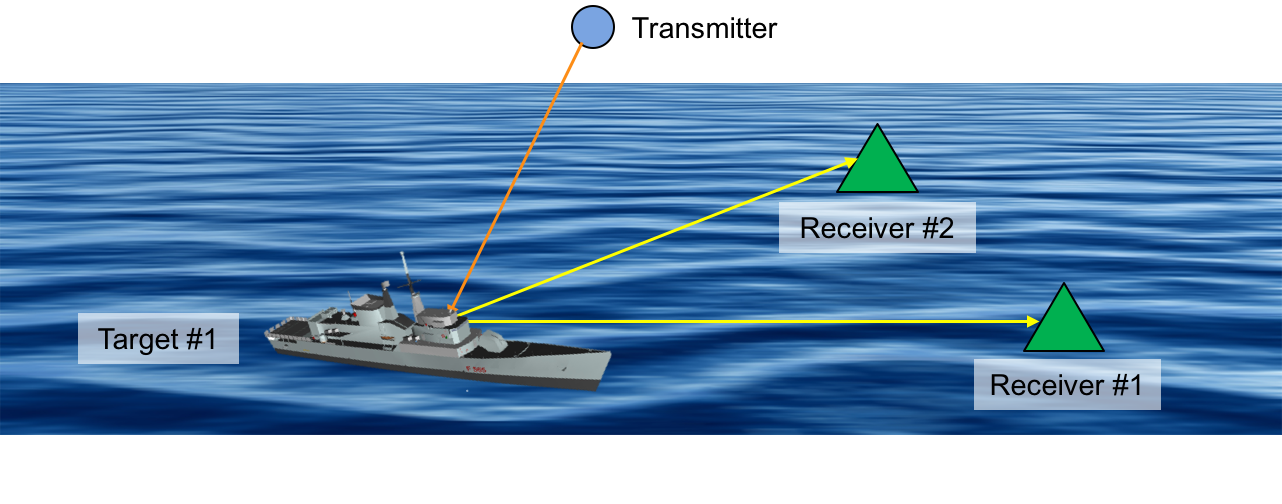
\includegraphics[width=5in]{../media/multistatic/ms_rf_concept.png}
  \end{center}
  \renewcommand{\baselinestretch}{1} \small\normalsize
  \begin{quote}
    \caption[Multistatic RF Sensor Networks Concept]{Multistatic RF Sensor Networks Concept\label{ms_fig:1}}
  \end{quote}
\end{figure}
\renewcommand{\baselinestretch}{2} \small\normalsize
Each receiver observes the target from a different aspect angle than it was illuminated with, resulting in different radiation patterns. The different paths between each receiver also means the impacts from multipath and clutter will be different. The initial goal will be to generate the statistics of the received signals through a Monte Carlo simulation by generating random realizations of the sea surface and numerically propagating the RADAR signal. Once we have the statistics, we can demonstrate that random matrix theory (RMT) predicts the signal PDFs and allows us a much faster method to evaluate RADAR system performance in a multistatic configuration. 

\section{Beam Width}
The beam width of an antenna is defined as the angle between the half power points in the antenna pattern.

\subsection{One Way}
The one way antenna beam width, $\theta$, is simply the beam width of the forward propagating beam.

\subsection{Two Way}
The two way antenna beam width, $\theta_2$, is the beam width of the return beam that propagates in both directions. For the monostatic case, we can compute this as the one way beam width of the square of the antenna pattern. In most cases, $\theta_2 \approx \frac{1}{\sqrt{2}}\theta$.

\section{RADAR Range Equation} 
The RADAR range equation provides a deterministic method to calculate received signal levels and is the workhorse for analyzing RADAR system performance. Thi equation is the first step towards building a statistical model, as it captures the underlying physics.


\subsection{Monostatic Case}
The RADAR range equation is derived by assuming spherically propagating waves and computing the propagated power at 4 incremental points between the transmitter and target as shown in Figure \ref{intro_fig:1}. These points are the projected power ($P_1$), the power received at the target ($P_2$), the power reflected by the target ($P_3$), and the power received back at the receiver antenna ($P_4$). The received power ($P_r$) is then the product with $P4$ and the effective area of the receiver antenna.

\begin{figure}[H]
  \begin{center}
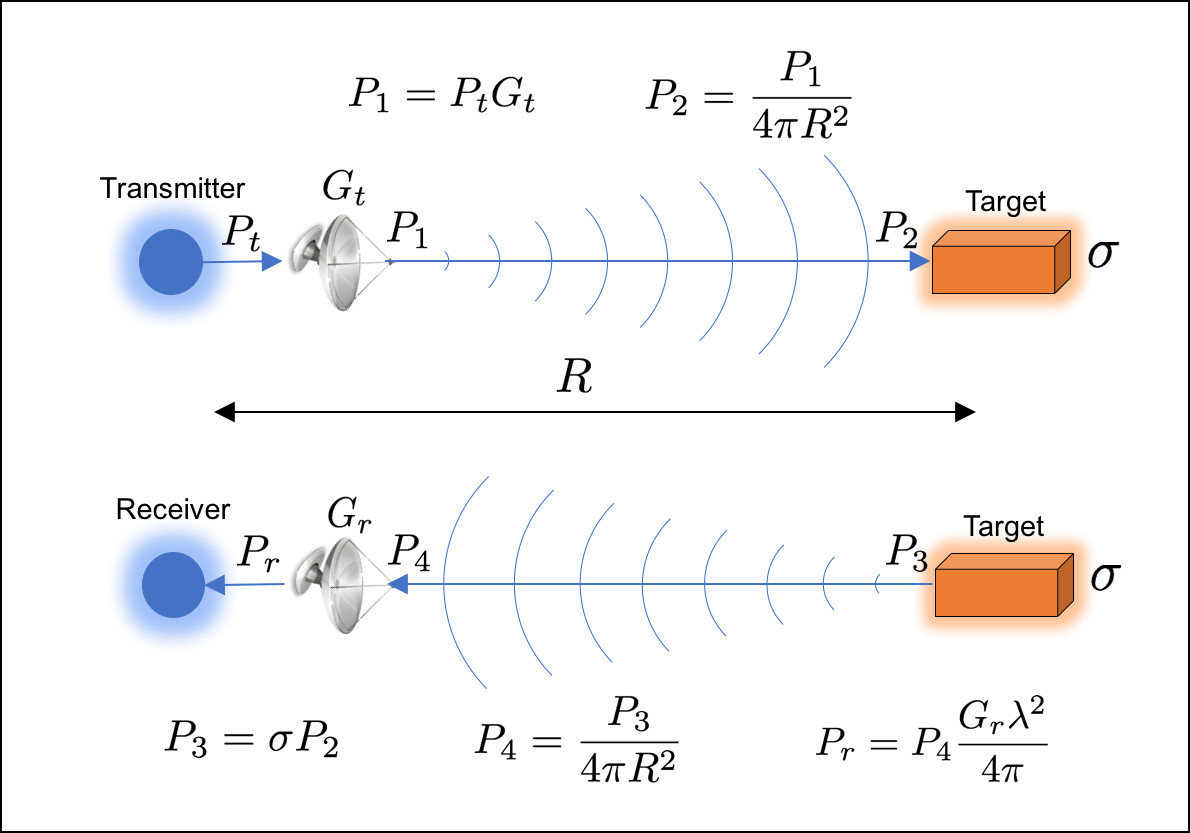
\includegraphics[width=4in]{../media/multistatic/radar_range_equation.png}
  \end{center}
  \renewcommand{\baselinestretch}{1} \small\normalsize
  \begin{quote}
    \caption[RADAR Range Equation Derivation]{RADAR Range Equation Derivation \label{intro_fig:1}}
  \end{quote}
\end{figure}
\renewcommand{\baselinestretch}{2} \small\normalsize

With spherical waves, the power is spread out over a sphere of radius equal to the slant range, $R$, which gives the factor of $\left( 4\pi R^2 \right)^{-1}$. The total projected power is the transmitted power, $P_t$, multiplied by the antenna gain, $G_t$. The RADAR cross section (RCS), $\sigma$, defines the amount of power intercepted and reflected. The effective area of the antenna is then $\frac{G_t\lambda^2}{4\pi}$.

The traditional monostatic RADAR range equation is shown in Equation \ref{intro_eq:1} \cite{skolnik_handbook}.
  \begin{equation}
  \label{intro_eq:1}
 P_r = \frac{P_tG_t^2\sigma\lambda^2}{\left(4\pi\right)^3R^4}
  \end{equation}

We can divide Equation \ref{intro_eq:1} by the noise power to represent the RADAR equation in terms of signal to noise ratio (SNR) as shown in Equation \ref{intro_eq:2} \cite{skolnik_handbook}.
\begin{equation}
    \label{intro_eq:2}
\text{SNR} = \frac{P_r}{P_n} = \frac{P_tG_t^2\sigma\lambda^2}{\left(4\pi\right)^3 R^4k_BTBF_n}
\end{equation}
In this equation, $k_B$ is the Boltzmann constant, $B$ is the receiver bandwidth, $T$ is the receiver temperature and $F_n$ is the receiver noise figure. Nominally, $B$ is taken to be the inverse of the pulse width to accomodate matched filter processing and $T$ is taken to be $300$ K.

\subsection{Bistatic Case}
In the bistatic case, we need to consider each path separately as the ranges, antenna gains, and RCS are all likely different. The standard bistatic RADAR range equation is shown in Equation \ref{intro_eq:3}.
  \begin{equation}
  \label{intro_eq:3}
 P_r = \frac{P_tG_tG_r\sigma_B\lambda^2}{\left(4\pi\right)^3R_1^2R_2^2}
  \end{equation}
In this equation, $G_t$ is the antenna gain for the transmitter, $G_r$ is the antenna gain for the receiver, $\sigma_B$ is the bistatic RCS, $R_1$ is the slant range along the first path, and $R_2$ is the slant range along the second path.

The bistatic RADAR range equation in terms of SNR is shown in Equation \ref{intro_eq:4}.
\begin{equation}
    \label{intro_eq:4}
\text{SNR} = \frac{P_tG_tG_r\sigma_B\lambda^2}{\left(4\pi\right)^3 R_1^2R_2^2k_BTBF_n}
\end{equation}

\subsection{Propagation Factors}
The use of a propagation factor, $F_p$, allows us to include atmospheric effects in the RADAR range equation. These effects can include absorption from atmospheric gases and weather such as rain or snow as well as rollups for the effects of multipath reflections, diffraction from the surface, and clipping by the horizon. The propagation factor is typically implemented as a multiplier to the RADAR range equation.

\section{Detection}
The detection process can be cast as a hypothesis test where the two mutually exclusive hypotheses are that the target is either present or not present \cite{richards_radar}. There are three probabilities that need to be considered. First, the probability of detection is the probability that a target is both detected and present. Second, the probability of false alarm, $P_{fa}$ is the probability that a target is detected but not actually present. Finally, the probability of miss, $P_m$ is the probability that a target is present but not detected. In most cases, a missed detection is worse than a false alarm.

\subsection{Probability of Detection}
The detection processes is generally a threshold test applied to the output of a matched filter generated for optimal detection with the threshold, $\hat{T}$ tuned to achieve a specified $P_{fa}$. For this section, we will assume the noise is zero mean, normally distributed  with variance $\beta^2$. 

\subsubsection{Coherent Receivers}
For coherent receivers, the phase of the signal is known. The threshold in this case is given in Equation \ref{intro_eq:5} and the $P_d$ is given in Equation \ref{intro_eq:6} \cite{richards_radar}.
\begin{equation} 
    \label{intro_eq:5}
\hat{T} = \sqrt{2N\beta^2}\text{erf}^{-1}(1-2P_{fa})
\end{equation}

\begin{equation}
    \label{intro_eq:6}
P_d = \frac{1}{2} \text{erfc}\left(\text{erfc}^{-1}(2P_{fa}) - \sqrt{\text{SNR}} \right)
\end{equation}

\subsubsection{Noncoherent Receivers}
For a noncoherent receiver, the phase of the signal is unknown and the threshold detector only operates on the magnitude of the signal. The threshold in this case is given in Equation \ref{intro_eq:7} \cite{richards_radar}.
\begin{equation}
    \label{intro_eq:7}
\hat{T} = \sqrt{-\beta^2 \ln{P_{fa}}}
\end{equation}

We can then define $P_d$ through Marcum's Q function, $Q_m$, for a given SNR and $P_{fa}$ as shown in Equation \ref{intro_eq:8} with $Q_m$ given in Equation \ref{intro_eq:9} \cite{richards_radar}.
\begin{equation}
    \label{intro_eq:8}
P_d = Q_m\left(\sqrt{2\text{SNR}}, \sqrt{-2\ln\left(P_{fa} \right)} \right)
\end{equation}

\begin{equation}
    \label{intro_eq:9}
Q_m(\alpha,\gamma) = \int_\gamma^\infty t\exp\left[-\frac{1}{2}(t^2 + \alpha^2) \right]I_0(\alpha t) dt
\end{equation}

\subsection{Processing Gains}
To improve the overall SNR and increase the $P_d$, we can take advantage of processing gains by applying the detection strategy to groups of pulses.

\subsubsection{Coherent Processing}
For coherent operation, we operate in the complex domain and add the magnitude and phase of each pulse.

\subsubsection{Noncoherent Processing}
For noncoherent operation, we only sum the magnitudes of each pulse.

\subsubsection{Binary Integration}